\documentclass[11pt]{article}
\usepackage{latexsym}
\usepackage{amsmath,amssymb,amsthm}
\usepackage{epsfig}
\usepackage[right=0.8in, top=1in, bottom=1.2in, left=0.8in]{geometry}
\usepackage{setspace}
\usepackage{graphicx}
\usepackage[numbers,sort]{natbib}

\usepackage{bm}
\usepackage{abstract}
\usepackage{algorithm}
\usepackage{algorithmic}
\usepackage{enumitem}
\usepackage{hyperref}
\usepackage{booktabs}
\usepackage{tabularx}
\setlist{nolistsep}
\spacing{1.25}

\newcommand{\handout}[5]{
  \noindent
  \begin{center}
  \framebox{
    \vbox{\vspace{0.25cm}
      \hbox to 5.78in { {SE3352:\hspace{0.12cm}Algorithm Design} \hfill #2 }
      \vspace{0.48cm}
      \hbox to 5.78in { {\Large \hfill #5  \hfill} }
      \vspace{0.42cm}
      \hbox to 5.78in { {#3 \hfill #4} }\vspace{0.25cm}
    }
  }
  \end{center}
  \vspace*{4mm}
}
\newcommand{\lecture}[4]{\handout{#1}{#2}{#3}{Scribes:\hspace{0.08cm}#4}{Notes #1}}

\newtheorem{theorem}{Theorem}
\newtheorem{corollary}[theorem]{Corollary}
\newtheorem{lemma}[theorem]{Lemma}
\newtheorem{observation}[theorem]{Observation}
\newtheorem{example}[theorem]{Example}
\newtheorem{definition}[theorem]{Definition}
\newtheorem{claim}[theorem]{Claim}
\newtheorem{fact}[theorem]{Fact}
\newtheorem{assumption}[theorem]{Assumption}
\newcommand{\E}{\textbf{E}}
\newcommand{\var}{\text{var}}
\def\eps{\ensuremath\epsilon}

\providecommand{\keywords}[1]{\textbf{{Keywords:}} #1}
\renewcommand{\abstractnamefont}{\Large\bfseries}

\begin{document}

\lecture{ -- Community Detection}{December 14, 2021}{Instructor:\hspace{0.08cm}\emph{Guoqiang Li}}{\emph{Zhemin Huang}, \emph{Xunjie Wang}}

\begin{abstract}
Community detection is an important and extremely useful tool in both scientific research and data analytics. This note offers a guided tour through the main aspects of community detection. We introduce several widely-used algorithms, ranging from traditional algorithms to state-of-the-art algorithms, which are mostly based on modularity. Besides, we point out the algorithm's application in industries. The challenges faced by community detection algorithms, open problems and future trends related to community detection are also discussed.

\end{abstract}

\keywords{community detection, network, community structure, modularity, deep learning}

\section{Introduction}
Nowadays, research on complex networks is getting more and more popular. A great variety of systems in nature, society or technology, can be modelled as networks. Community detection, or more specifically, \textbf{clustering nodes based on similar features}, helps us understand the inherent patterns and functions of networks.

\noindent Researchers have proposed many community detection algorithms with different types and scale of complex networks. However, there are still no universal guidelines on how to assess the performance of different algorithms, or compare them with each other. Traditionally, modularity is preferred by most mainstream algorithms. With the era of deep learning coming, new algorithms and problems are being discussed as well.

\noindent This note is composed as follows. We introduce some related concepts of community detection in Section 2. In section 3, we introduce some key properties of the basic concept -- modularity. In section 4-7, we introduce several algorithms of different levels, and parallel implementation in industries. 
In section 8-9, we discuss community detection's real applications, and its future directions.


\section{Problem Description}

In this section, we first define two simple concepts: network and community. \\A network is a special graph that abstracts \textbf{complex relationships} in real-world systems, such as Internets, social networks, or biological cell architecture.

\begin{definition}
  [Network]
  A weighted network is represented as $G=(V,E,W)$, and an unweighted network is represented as $G=(V,E)$, where $V,E$ denote the set of nodes and edges, respectively, and $W$ denotes the corresponding weights of the connections.
  In an unweighted network, $W$ can be regarded as 1 and can be removed from $G$. Besides, a network is either a directed graph, or an undirected graph.
\end{definition}
\noindent A community is a type of sub-graph that represents some real social phenomenon. In order words, a community is a group of people or objects, which \textbf{share common characteristics}.
\begin{definition}
  [Community]
  Communities are the sub-graphs in a network, where nodes share dense connections. Sparsely-connected nodes cripple communities. 
  We use $C=\{C_1,C_2,...,C_k\}$ to denote a set of $k$ communities divided from a network $G$. A node $v$ clustered into the community $C_i$ satisfies the condition that the internal degree of each node inside the community exceeds its external degree. For $\forall i,j, C_i\in C, C_j\in C$, they satisfy the following conditions
  \begin{equation}
        C_i\cap C_j=\varnothing
  \end{equation}
  \begin{equation}
    \bigcup_{i=1}^{k}C_i=G
  \end{equation}
  % A node $v$ clustered into the community $C_i$ satisfies the condition that the internal degree of each node inside the community exceeds its external degree.
\end{definition}
% It is obvious that community detection is similar to clustering problems.
\noindent Modularity was designed to measure the strength of division of a network into communities. It was proposed by Newman.\cite{newman2004}  
\begin{definition}
  [Modularity]
  Consider a particular division of a network into $k$ communities. Let us define a $k \times k$  symmetric matrix $e$ whose element $e_{ij}$ is the fraction of all edges in the network that link vertices in community $i$ to vertices in community $j$.
  We further define the row sums $a_i=\sum_{j}e_{ij}$, which represent the fraction of edges that connect to vertices in community $i$.
  In a network in which edges fall between vertices who belong to different communities, we would have $e_{ij}=a_ia_j$. Let $||X||$ indicates the sum of the elements of the matrix $X$.
  Thus, we define modularity by
  \begin{equation}
    Q=\sum_i{e_{ii}-{a_i}^2}=\sum_i{e_{ii}}-\sum_i{{a_i}^2}=Trace-||e^2||
  \end{equation}
\end{definition}
\noindent If $Q$ is high, we get strong community structure. In practice, values for such networks typically fall in the range from about 0.3 to 0.7.\cite{newman2004}

\noindent In order to raise \textbf{a spectral algorithm for community detection}, Newman redefined the concept of modularity.\cite{newman2006}
\begin{definition}
  [Reformulation of the modularity]
  The modularity of a community partition is a scalar ranging from $-\frac{1}{2}$ to $1$ that evaluates the density of links inside communities as compared to links between communities.
For a given graph $G = (V, E)$. Let $A_{ij}$ be the weight of the edge between $i$ and $j$, $k_{i} = \sum_{(i, j) \in E}A_{ij}$ is the sum of the weights of all the edges attached to vertex $i$,  $m = \frac{1}{2}\sum_{ij}A_{ij}$, the quantity $\frac{1}{2}(s_is_j+1)$ is 1 if $i$ and $j$ are in the same group and 0 otherwise,
\begin{equation}
  \begin{split}
    Q = \frac{1}{4m}\sum_{i \in V, j \in V}(A_{ij} - \frac{k_{i}k_{j}}{2m})\frac{1}{2}(s_is_j+1)
  \end{split}
\end{equation}
\end{definition}
\noindent The leading factor of $\frac{1}{4m}$ seems to be confusing. Actually, it is included for compatibility with the previous definition of modularity.

\noindent From the definitions above, we can lead to our goal--community detection.
\begin{definition}
  [Community detection]
  Community detection is a method to extract communities from large networks when the modularity is optimal.
\end{definition}
\noindent We need to point out that not all methods are based on modularity, such as Infomap\cite{infomap2008}. Modularity has its limits\cite{resolution2007}, but it is still the most commonly used method for evaluating results. 

\section{Key Properties}
In this section, we introduce some key properties of modularity, which helps to understand following algorithms.

\begin{lemma}
  We denote the set of all possible communities of a graph $G$ with $A(G)$, $Q(P)$ refers to the modularity of $P$. 
  Let $G$ be an undirected and unweighted graph and $P \in A(G)$. Then $-\frac{1}{2}\le Q(P) \le 1$ holds.
  \begin{proof}
    Let $m_i=|E(P)|$ be the number of edges inside community $P$ and $m_e=\sum_{P\neq P'\in P}|E(P, P')|$ be the number of edges having exactly one end-node in $P$. Then we can calculate the contribution of $P$ to $Q(P)$
    \begin{equation}
      \frac{m_i}{m}-(\frac{m_i}{m}+\frac{m_e}{2m})^2=\frac{-4(m_i)^2+4m_i(m-m_e)-(m_e)^2}{4m^2}
    \end{equation}
    It is obvious that the only maximum point is at $m_i=\frac{m-m_e}{2}$. The contribution of a community is minimized when $m_i$ is zero and $m_e$ is as large as possible.
    Suppose now $m_i=0$, the upper bound can only be actually attained in the specific case of a graph with no edges, where coverage is defined to be 1.
    Besides, any bipartite graph $K_{a,b}$ with simple communities $C=\{C_a, C_b\}$ yields the minimum modularity of $\frac{1}{2}$. This proof the lemma.
  \end{proof}
\end{lemma}

\begin{theorem}
  Modularity is \textbf{NP-complete}.\cite{brandes2007modularity}
  \begin{proof}
    We formalize the problem of finding modularity, and prove it by \textbf{reduction}.
    \\ \textbf{Problem 1 (Modularity) }: Given a graph $G$ and a number $K$, is there a community $P\in G$, for which $Q(P)\ge K$? ($K\in [-\frac{1}{2},1]$)
    \\ \textbf{Problem 2 (3-Partition) }: Given $3k$ positive integer numbers $a_1,...,a_{3k}$ such that the sum $\sum_{i=1}^{3k}a_i=kb$, and $\frac{b}{4} < a_i < \frac{b}{2}$, for an integer $b$ and for all $i=1,...,3k$,
    is there a partition of these numbers into $k$ sets, such that the sum of the numbers in each set equals to $b$?
    \\ It has been proved that 3-partition problem is a NP-Complete problem.\cite{provenp}
    \\ Then we show that an instance $A={a_1,...,a_{3k}}$ of 3-partition problem can be transformed into an instance $G(A), K(A)$ of modularity problem.
    \\ Given an instance $A$ of 3-partition, we can construct a graph $G(A)$ with $k$ cliques $H_1,...,H_k$ of size $a=\sum_{i=1}^{3k} a_i$ each. For each element $a_i\in A$, we introduce a single element node in graph, and 
    connect it to $a_i$ nodes in each of the $k$ cliques, where each clique member is connected to exactly one element node. Therefore, each clique node has degree $a$, and the element node corresponding to element $a_i\in A$ has degree
    $ka_i$. The number of edges in $G(A)$ is $m=\frac{k}{2}·a(a+1)$.
    \\ Then we construct $K(A)$. Since graph $G(A)$ has exactly $k$ cliques, it has exactly $(k-1)a$ inter-community edges, so the edge contribution is given by
    \begin{equation}
      \begin{split}
      \sum_{C\in P}\frac{|E(C)|}{m}=\frac{m-(k-1)a}{m}
      \end{split}
      \begin{split}
      =1-\frac{2(k-1)a}{ka(a+1)}=1-\frac{2k+2}{k(a+1)}
      \end{split}
    \end{equation}
    Therefore, communities $P=(C_1,...,C_k)$ with maximum modularity must minimize $d(C_1)^2+d(C_2)^2+...+d(C_k)^2$, where $d(C_k)$ refers to the degree of $C_k$. Then the sum of degrees per community should be as small as possible.
    In the optimum case, we can assign to each community element nodes corresponding to elements that sum to $b=\frac{1}{k}·a$. In each clique, the sum equals to $k·\frac{1}{k}·a=a$. 
    \begin{equation}
      d(C_1)^2+...+d(C_k)^2\ge k(a^2+a)^2 = ka^2(a+1)^2
    \end{equation}
    Hence, if there exist communities $P$ with $Q(P)$, then 
    \begin{equation}
      K(A)\ge 1-\frac{2k-2}{k(a+1)}-\frac{ka^2(a+1)^2}{k^2a^2(a+1)^2} = \frac{(k-1)(a-1)}{k(a+1)}
    \end{equation}
    As each element node is contained in exactly one community, this yields a solution for the instance of 3-partition. The instance of 3-partition is satisfiable if the instance of modularity is satisfiable.
    \\Otherwise, suppose the instance for 3-partition is satisfiable. Then there exists a partition into $k$ sets, where the sum over each set is $\frac{1}{k}·a$. If we detect communities by joining the element nodes of each set with a different clique, we get communities of modularity $K(A)$. Therefore, the instance of modularity is satisfiable if the instance of 3-partition is satisfiable.
    \\Therefore, the theorem holds.
  \end{proof}
\end{theorem}


\section{Girvan-Newman Algorithm}

\subsection{Introduction}

Girvan-Newman algorithm is the first algorithm of the modern age of community detection in graphs.\cite{newman2006} 
It is a hierarchical divisive method, in which links are iteratively removed based on the value of their betweenness, which expresses the number of shortest paths between pairs of nodes that pass through the link. 
In the most popular implementation, the procedure of link removal ends when the modularity of the resulting partition reaches a maximum.

\linespread{1.25}\selectfont
We can describe Girvan-Newman algorithm in the following way:
\begin{itemize}
  \setlength{\topsep}{0pt}
  \setlength{\itemsep}{1.25pt}
  \setlength{\parsep}{1.25pt}
  \setlength{\parskip}{1.25pt}
  \item [1)] Calculate edge betweenness for every edge in the graph.
  \item [2)] Remove the edge with the highest edge betweenness.
  \item [3)] Calculate edge betweenness for remaining edges.
  \item [4)] Repeat steps 2-4 until all edges are removed.
\end{itemize}


\subsection{Edge Betweenness}

\begin{definition}
  [Edge Betweenness]
  the edge betweenness of $(i,j)$ is the number of the shortest paths between pairs of vertices that pass through the edge $(i,j)$.

\end{definition}

For a given graph $G = (V, E)$, Let $d_{s, i}$ be the length of the shortest path between vertex $s$ and vertex $i$, $w_{s, i}$ be the number of the shortest paths from vertex $s$ to vertex $i$, $b_{s, i}$ be the number of the shortest paths between vertex $s$ to any vertex in graph that pass through vertex $i$. Edge betweenness $\sigma_{i,j}$ of edge $(i,j)$ can be computed by:

\begin{equation}
  \begin{split}
    \sigma_{i,j} = \sum_{s \in V}\sigma_{s,i,j}
  \end{split}
\end{equation} where
\begin{equation}
  \begin{split}
    \sigma_{s,i,j} = \begin{cases}
      \frac{w_{s,j}}{w_{s,i}}b_{s,i} & d_{s,i} > d_{s,j} \\
      \frac{w_{s,i}}{w_{s,j}}b_{s,j} & d_{s,i} < d_{s,j} \\
      0                              & d_{s,i} = d_{s,j}
    \end{cases}
  \end{split}
\end{equation}

\subsection{Method}

For each source vertex $s$, we can compute the triple $(d_{s, i}, b_{s, i}, w_{s, i})$ as follows.\cite{newman2006}

The first part of the algorithm for vertex marking:
\begin{itemize}
  \item [1)] For initial vertex $s \in V$, let $d_{s,s}=0, w_{s,s}=1, b_{s,i}=0$.
  \item [2)] Let $d_{s,v}$ = $\infty$, $w_{s,v}=0, b_{s,v}=1$ for all $v \neq s \in V$ .
  \item [3)] Create queue $Q$, $Q \leftarrow \{s\}$. Create list $L$, $L \leftarrow \{s\}$.
  \item [4)] While $Q$ is not empty:
        \begin{itemize}
          \item [a)] Dequeue $i \leftarrow Q$.
          \item [b)] For each vertex $j$ where $(i,j)\in E$
                \begin{itemize}
                  \item [i)]   If $d_{s,j}=\infty$ then $d_{s,j} = d_{s,i}+1, w_{s,j} = w_{s,i}$. Enqueue $j \rightarrow Q$. Push $j \rightarrow L$.
                  \item [ii)]  If $d_{s,j} \neq \infty$ and $d_{s,j} = d_{s,i}+1$ then $w_{s,j} = w_{s,j}+w_{s,i}$.
                  \item [iii)] If $d_{s,j} \neq \infty$ and $d_{s,j} < d_{s,i}+1$ then do nothing.
                \end{itemize}
        \end{itemize}
\end{itemize}
For each source vertex $s$, each edge will be visited twice. Therefore, the time complexity of this part of the algorithm is $O(mn)$.

\noindent The second part of the algorithm starts from the vertex that was last marked in the first part of the algorithm and visits vertices in reverse order than they were visited in the first part of the algorithm:
\begin{itemize}
  \item [1)] While $L$ is not empty:
        \begin{itemize}
          \item [a)] Pop $i \leftarrow L$.
          \item [b)] For each vertex $j$ where $(i,j)\in E$
                \begin{itemize}
                  \item [i)]  If $d_{s,i} < d_{s,j}$ then $b_{s,i} = 1+\sum_{j}\sigma_{s,i,j}$.
                  \item [ii)] If $d_{s,i} > d_{s,j}$ then $\sigma_{s,i,j} = \frac{w_{s,j}}{w_{s,i}}b_{s,i}$.
                \end{itemize}
        \end{itemize}
\end{itemize}
Similar to the first part, the time complexity of this part of the algorithm is also $O(mn)$.

\noindent Each edge will be removed only once. Therefore, the time complexity of the whole algorithm is \bm{$O(m^2n)$}.

% \subsection{Modularity}

% The Modularity of a community partition is a scalar ranging from $-\frac{1}{2}$ to $1$ that evaluates the density of links inside communities as compared to links between communities.


% For a given graph $G = (V, E)$. Let $A_{ij}$ be the weight of the edge between $i$ and $j$, $k_{i} = \sum_{(i, j) \in E}A_{ij}$ is the sum of the weights of all the edges attached to vertex $i$,  $m = \frac{1}{2}\sum_{ij}A_{ij}$,

% \begin{definition}
%   [Modularity]
%   the modularity of $G$
%   \begin{equation}
%     \begin{split}
%       Q = \frac{1}{2m}\sum_{i \in V, j \in V}[A_{ij} - \frac{k_{i}k_{j}}{2m}]
%     \end{split}
%   \end{equation}

% \end{definition}

% Modularity can give an answer to when an optimal decomposition of a network into communities is reached.
% Girvan-Newman algorithm computes the modularity of current community partition, and determined to terminate when the modularity of the resulting partition reaches a maximum.

\subsection{Conclusion}

Girvan-Newman algorithm is an intuitive algorithm and easy to implement, which can produce correct classifications of vertices in small networks. 

\noindent But the time complexity is $\bm{O(m^2n)}$, or $\bm{O(n^3)}$ for sparse networks, which limits performance on gigantic networks.\cite{newman2006} 

\noindent A greedy algorithm, which will be discussed later, can give much smaller complexity than Girvan-Newman algorithm.

\section{Louvain Algorithm}

\subsection{Introduction}

Fast unfolding of communities in large networks, also known as Louvain algorithm\cite{louvain}, is a heuristic optimization algorithm of community detection based on the modularity of the given graph. The algorithm performs better in terms of efficiency and effectiveness, and can discover the hierarchical community structures. The goal of optimization is to maximize the modularity of the entire community network.

\subsection{Method}

The Louvain algorithm is composed of two iteration phases. Initially, each vertex in the network will be considered as an individual community.

\noindent In the first phase, for each vertex $i$, consider the change of modularity $\Delta{Q}$ when removing vertex $i$ from its community and then placing it to the community of its neighbor $j$. This action will be executed only if $\Delta{Q}$ is positive and is the maximal $\Delta{Q}$ of all adjacent of vertex $i$. Obviously, the first phase will terminate when $Q$ reaches the local maxima.

\noindent This removing-placing action can be decomposed into two similar actions: making vertex $i$ isolated and moving the isolated vertex into a community. The removing action is just the inverse action of placing action. Let $\sum_{in}$ be the sum of the weights of the internal edges of $c_{j}$, $\sum_{tot}$ be the sum of the weights of the links incident to vertices in community $c_{j}$, $k_{i, in}$ be the sum of the weights of the links from $i$ to vertices in community $c_{j}$. When moving an isolated vertex $i$ into a community $c_{j}$, the change of modularity can be easily computed by:
\begin{equation}
  \begin{split}
    \Delta{Q} = \bigg[\frac{\sum_{in} + k_{i, in}}{2m} - \bigg(\frac{\sum_{tot} + k_{i}}{2m}\bigg)^{2}\bigg] - \bigg[\frac{\sum_{in}}{2m} - \bigg(\frac{\sum_{tot}}{2m}\bigg)^{2} - \bigg(\frac{k_{i}}{2m}\bigg)^{2}\bigg]
  \end{split}
\end{equation}
Fortunately, $\sum_{tot}$, $\sum_{in}$ and $k_{i, in}$ can be easily maintained during the iteration.

\noindent In the second phase, the whole network will shrink to a new network whose vertices are the communities generated by the first phase. The weights of edges between two new vertices are determined by sum of the weights of the edges between vertices in the corresponding two communities. The internal edges of a community leads to a self-loop for the corresponding vertex in the new network. The second phase will generate a new network that is possible to reapply the algorithm in the first phase, and then the algorithm will go to next iteration.

\noindent Let us denote by "pass" a combination of these two phases. The passes will keep being iterated until convergence of the modularity $Q$. Figure \ref{fig:louvain} shows the visualization of the Louvain algorithm with a simple graph. As discussed before, the Louvain algorithm can discover the hierarchical structures of communities of the network. The height of hierarchical community structure is equal to the number of passes, which is empirically a small number in common cases.

\begin{algorithm}
	\caption{Pseudocode of the Louvain algorithm\cite{aynaud2010static}}
	\label{louvain_code}
	\begin{algorithmic}
		\REQUIRE {the initial network $G=(V,E)$}
		\ENSURE {final community assignment $C$, and modularity $Q$}
		\REPEAT
		\STATE {Put each node of $G$ in its community}
		\STATE {$Q' \leftarrow Q $}
		\WHILE{some nodes are moved}
		\FOR{$v \in G$}
		\STATE {Place $v$ in its neighboring community including its own, which maximizes the modularity gain}
		\ENDFOR
		\ENDWHILE
		\STATE {Calculate new modularity $Q$}
		\IF{$Q > Q' $}
		\STATE {$C \leftarrow$ the network between communities of $G$}
		\ELSE 
		\RETURN {$C,Q$}
		\ENDIF
		\UNTIL {true}
	\end{algorithmic}
\end{algorithm} 

\begin{figure}[p]
  \centering
  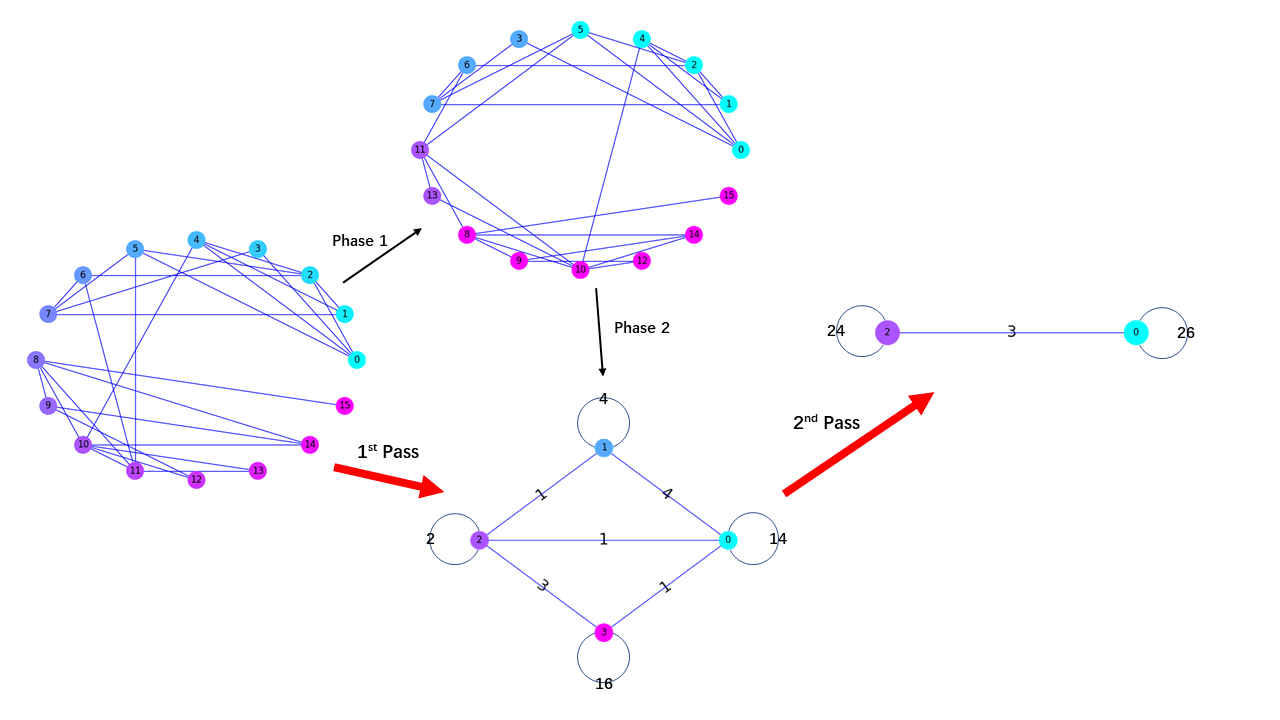
\includegraphics[scale=0.5]{figures/louvain.png}
  \caption{Visualization of the steps of Louvain algorithm. The first phase is to optimize the modularity using a heuristic approach. The second phase is to aggregate vertices in one community into a super vertex, in order to generate a new network possibly for reapplying the first phase. When the network can not gain modularity anymore, the whole algorithm terminates.}
  \label{fig:louvain}
\end{figure} 

\subsection{Conclusion}

The Louvain algorithm is an intuitive heuristic algorithm, which is a multistep technique based on a local optimization of Newman-Girvan modularity in the neighborhood of each node. Due to the easy computation of $\Delta{Q}$ and swift convergence of $Q$, the whole algorithm runs extremely fast. Many experiments suggest that its complexity is linear on typical and sparse data.  

\section{Parallelization of Louvain algorithm}

In the original serial algorithm, each vertex examines the communities of its neighbors and makes a choice to chooses a new community based on a function to maximize the calculated change in modularity.
In the distributed version all vertices make this choice simultaneously rather than in serial order, updating the graph state after each change. Because choices are made in parallel some choice will be incorrect and will not maximize modularity values, however after repeated iterations community choices become more stable and can give an approximate result closely mirror the serial algorithm.

\subsection{Implementation}

Practically, It is a good choice to implement a parallel algorithm on Spark.\cite{spark} Spark is a cluster computing framework supporting reusing a working set of data across multiple parallel operations while retaining the scalability and fault tolerance of MapReduce.\cite{mapreduce} The implementation of parallelization of Louvain on Spark is described as:
\begin{itemize}
  \item [1)] Consider each vertex in the graph as an independent community.
  \item [2)] For each vertex $i$, remove the vertex $i$ from the original community and assign it to one of the communities of its adjacent vertices, calculate the modularity increment after vertex $i$ is assigned to the new community, and record the adjacent vertex with the maximal modularity increment. If the modularity increment is positive, add vertex $i$ to the community where the adjacent vertex corresponding to the maximal modularity increment Otherwise it remains unchanged.
  \item [3)] Repeat 2) in parallel until the structure of communities no longer changes.
  \item [4)] Merge vertices in the same community into new vertices and update weights of edges in parallel.
  \item [5)] Repeat 1) in parallel until the modularity of the whole network no longer changes.
\end{itemize}

To describe using MapReduce:
\begin{itemize}
  \item [1)] Get information of adjacent vertices.
        \begin{itemize}
          \item [a)] Map: produce information of adjacent vertices $\text{VertexData}$;
          \item [b)] Reduce: get information of adjacent vertices $(\text{Id}, \text{Array}[\text{VertexData}])$.
        \end{itemize}
  \item [2)] Get the new community of every vertices $(\text{Id}, \text{getBestCommunity}(\text{Array}[\text{VertexData}]))$
  \item [3)] Update the information in the network and merge vertices to go to next iteration.
\end{itemize}

\subsection{Conclusion}

Parallelization can effectively improve the efficiency of Louvain algorithm. This is because it makes full use of the excellent performance of parallel computing in iterative computing when computing information attached to vertices, combined with the distributed computing model, which greatly reduce computing time.

\section{Improvement of Louvain Algorithm}
\subsection{Drawbacks of Louvain Algorithm}
The Louvain algorithm is very simple and elegant, however, it has some \textbf{crucial drawbacks}. 

\noindent In the Louvain algorithm, a node may be moved to a different community, while it may have acted as a "bridge" between different communities. Removing such a node disconnects the nodes in the old community. 

\noindent An expected result is that other nodes in the old community will then be assigned to other communities. However, this is not necessarily the case. Figure \ref{fig:drawback} has elucidated such situation.
\begin{figure}[ht]
  \centering
  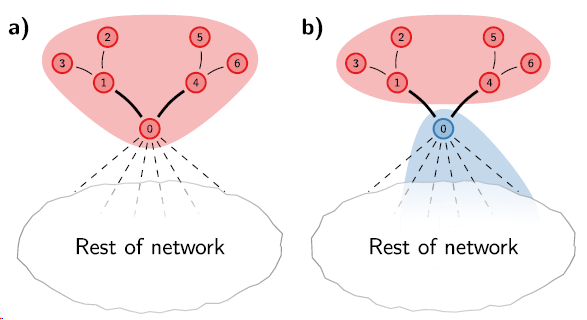
\includegraphics[scale=0.75]{figures/louvain_drawback.png}
  \caption{Disconnected community. When node 0 in ($a$) is moved to a different community, the red community becomes internally disconnected, as shown in ($b$). However, node 1-6 will still stay in the red community, which is not a satisfying result.\cite{leiden}}
  \label{fig:drawback}
\end{figure}

\subsection{Leiden Algorithm}
\renewcommand\arraystretch{1.5}
The Leiden algorithm was named after the university's name, and was designed to solve the problems of the Louvain algorithm.\cite{leiden}
The Leiden algorithm is more complex than the Louvain algorithm. It consists of three phases:
\begin{itemize}
  \item [1)] Local moving of nodes.
  \item [2)] Refinement of the partition.
  \item [3)] Aggregation of the network based on the refined partition, use the non-refined partition to create an initial partition for the aggregate network.
\end{itemize}
\noindent From figure \ref{fig:leiden}, we can have an intuitive understanding of the whole process.
\begin{figure}[ht]
  \centering
  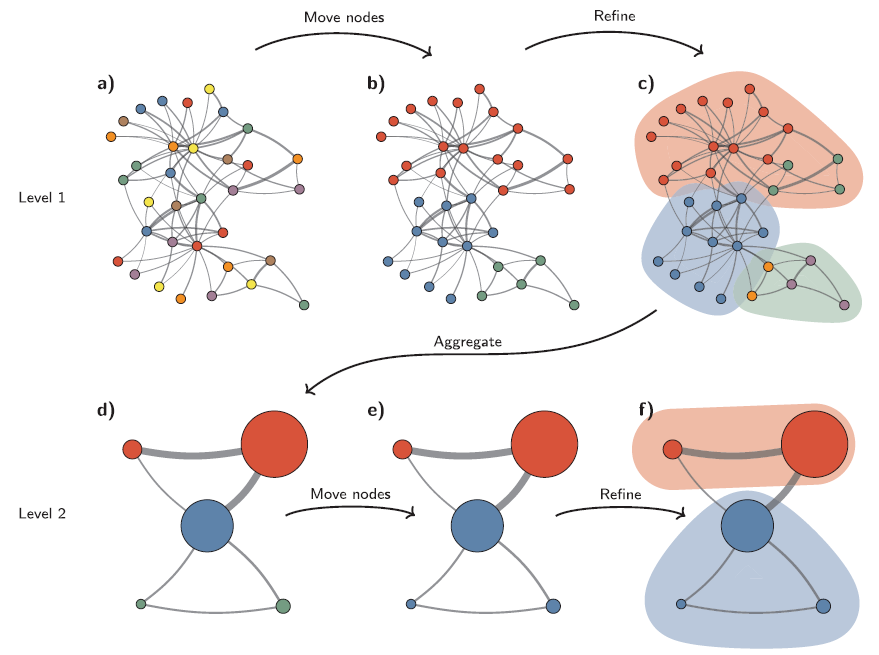
\includegraphics[scale=0.6]{figures/leiden.png}
  \caption{Leiden algorithm. The Leiden algorithm starts from a singleton partition ($a$). The algorithm moves individual nodes from one community to another to find a partition ($b$), which is then refined ($c$). An aggregate network ($d$) is created based on the refined partition, using the non-refined partition to create an initial partition for the aggregate network. For example, the red community in ($b$) is refined into two subcommunities in ($c$), which after aggregation become two separate nodes in ($d$), both belonging to the same community. The algorithm then moves individual nodes in the aggregate network ($e$). In this case, refinement does not change the partition ($f$). These steps are repeated until no further improvements can be made.\cite{leiden}}
  \label{fig:leiden}
\end{figure}

\noindent The algorithm has been widely accepted and used. For example, \textbf{scanpy} is a well-known python package for analyzing single-cell gene expression data.\cite{scanpy} Developers have replaced the default community detection method with Leiden algorithm, which has better performance on large-scale data.


\subsection{Conclusion}
The Leiden algorithm is an improved version of the Louvain algorithm, which is also the \textbf{state-of-the-art} algorithm. It is more complicated than Louvain algorithm, but has better compatibility and efficiency.
Table \ref{tab:compare} shows the comparison of the Louvain and Leiden algorithm.
\begin{table*}[!htbp]
	\centering
	\caption{Comparison between Louvain and Leiden algorithm}
	\begin{tabularx}{\textwidth}{lXXX}
		\toprule
		&  \textbf{Louvain} & \textbf{Leiden}  \\
		\midrule
  Year            & 2008& 2019\\
  Proposed by     & Blondel et al.& V.A. Traag et al.\\
  Phase           & 2 & 3 \\
  Advantage(s)    & $\bullet$ Performs well on small and medium-scale networks.  &  $\bullet$ Higher quality function, less time to run. \\
                  & $\bullet$ Static networks.   & $\bullet$ Temporal networks. \\
                  &                    & $\bullet$ The community are well-connected when running the algorithm iteratively. \\ 
  Disadvantage(s) & $\bullet$ Communities are badly connected or disconnected, especially when running the algorithm iteratively.  & $\bullet$ Extra step in the process.  \\
                  & $\bullet$ Disable detect in overlapping community. & \\
		\bottomrule
	\end{tabularx}
	\label{tab:compare}
\end{table*}

\section{Applications of community detection}
The goal of community detection algorithms is to deduce the properties and relationship of nodes, which is not possible from direct observations/measurements.
This section explores what can be done by using community detection algorithms. 

\noindent There are many networks such as social networks, informational networks, biological networks, and even
economic networks, where community detection is playing an important role.

\subsection{Applications in Social Networks}
Social networks are getting more and more popular today. An online social network is the interaction of people with each other through the web. Community detection has been widely used in this area.

\noindent \textbf{Twitter} is a popular social networking service around the world. Various studies have utilized different community detection methods to analyze public emotional reaction and visualize user relationships and characteristics. 
Researchers analyzed the reactions of Twitter users on the social and political issues. They used a community-based model to analyze and predict how these big events can influence users.\cite{twitter2009}
In another work, researchers used non-negative matrix factorization framework to cluster the politically inclined users on Twitter network into political communities.\cite{twitter2016}

\noindent During \textbf{crisis situations}, people often use social media to seek for help. Researchers have used a large scale contextualized community detection to find and recommend potential and relevant collaborators through social media, which has good time performance as well.\cite{crisis2015}

\subsection{Applications in Biological Networks} 

\textbf{Proteins} have unique and complicated structures, which can be divided into functional modules and protein complexes.\cite{chen2014} These two parts of proteins have been explored in various studies. Researchers have used simple Girvan-Newman algorithm to detect functional modules in protein-protein interaction networks.\cite{protein2005}
Besides, Protein constitutes the fundamental material of human's brain cells. Therefore, community detection can also been applied to \textbf{neurosciences} to study brain networks and even find the mechanism of Alzheimer's disease.\cite{neuro2017}

\noindent In another research, researchers have proposed an algorithm called \textbf{disease-gene network detecting algorithm}, based on Principal Component Analysis (PCA), 
which can extract the communities in a bipartite network.\cite{disease2013} This algorithm is aimed at disease prevention and medical diagnosis.


\subsection{Applications in Economics}
In economics and financial data analysis, it is important to categorize companies based on their economic value, stock price, current achievement, etc. 

\noindent In the \textbf{stock market}, each stock can be represented by a vertex and edge represents the correlations of stock values in the market. Researchers have stated the way to construct the network of stock market and detect communities in it. They revealed community structure by using modularity $Q$, which helps to the analysis and decision-making of the stock market.\cite{stock2014}

\subsection{Other Applications}
Besides having applications mentioned above, community detection has various general application. 

\noindent For example, community detection is also being employed for \textbf{refactoring of software packages}.
Refactoring is an effective way to improve the quality of the existing code. Researchers have presented a novel method to refactor object-oriented software package structure by using classes and their dependencies in software networks\cite{software2018}, which has been used in a lot of modern integrated development environments (IDE).

\section{Conclusion}
In this note, we have discussed some key properties, presented several commonly used algorithms and highlighted the industrial application of Louvain algorithm.
We also reviewed the multidisciplinary applications of community detection in various domains such as sociology, biology, economics, software engineering, etc. 
However, there are still some questions left to be discussed.
\subsection{Future Direction}
\textbf{Deep learning} is absolutely a promising direction of community detection. Beyond simply examining network topologies for detecting communities, some strategies also explore semantic descriptions as node features in the data. 

\noindent Recent researches have modified deep learning models based on community properties, and got promising results.\cite{deep2019}
Through a transitional graph embedding method, node distributions could be used to preserve the network structure to improve community detection in reverse.

\noindent \textbf{Temporal analysis of community detection} is also a future direction. Real world networks evolve over time, and the communities in such networks also change accordingly.
Therefore, exploiting temporal characteristics are crucial to learn deep insights about the communities.

\subsection{Open Problems}
In this section, we discuss several broad challenges, or the longest standing issue in community detection.

\subsubsection{Network Dynamics}
Changing dynamics can affect either the network topology or the node attributes. Topological changes, such as adding or deleting a node or edge, not only cause changes in a local community, but also leads to devastating changes across an entire network.
With dynamic networks, we need to recalculate the whole graph over a series of snapshots. The technical challenge lies in the deep feature extraction of dynamic networks.

\noindent Actually, a lot of methods have been used to deal with sequential data in machine learning, such as long short-term memory (LSTM).\cite{lstm} Therefore, deep learning methods for detecting communities with dynamic spatial and temporal properties are very likely to be developed. 

\subsubsection{Large-scale Networks}
Nowadays, large-scale networks can contain millions of nodes, edges, and structural patterns, as networks like Twitter and Weibo, which has also brought a lot of problems. 
For instance, large-scale networks may have their inherent characteristics, such as \textbf{scale-free}. There exists lots of mega hubs in the network, which can influence the performance of algorithms in community detection.

\noindent Besides, scalability seems to be another tricky problem to detect communities in large-scale networked environments.

% \subsubsection{Hierarchical networks}
% Hierarchical networks are made of layered networks, where each layer of networks share specified functions. Therefore, the community detection strategy must be able to extract layer-wise representations.
% The challenges include distinguishing different relationship types in the network, and make wise classifications.

\subsubsection{Number of Communities}
In fact, most algorithms of the community detection require the \textbf{number of communities} beforehand as a hyperparameter, including deep learning. 

\noindent There exist two approaches for the estimation of the number of communities in a network. One method is using modularity-based algorithm, like Girvan-Newman algorithm, and other one is based on \textbf{statistical interference}, which is also proposed by Newman.\cite{newman2016}
However, both methods have poor performance under large-scale networks.

\nocite{*}
\bibliographystyle{acm}
\bibliography{ref.bib}



\end{document}
